% P17 WORKING STANDALONE REPORT ENTRY POINT
% Compile from project/report with XeLaTeX, then BibTeX, then XeLaTeX twice.
% Original template templates/original/ is PRESERVED, not overwritten.
% This is NOT institutional-template-approved, NOT proof of final research readiness.
\documentclass[a4paper,12pt,oneside]{report}
\usepackage{fontspec}
\IfFontExistsTF{TeX Gyre Termes}{\setmainfont{TeX Gyre Termes}}{\setmainfont{DejaVu Serif}}
\usepackage[vietnamese]{babel}
\usepackage[a4paper,left=30mm,right=25mm,top=25mm,bottom=25mm]{geometry}
\usepackage{amsmath,graphicx,array}
\usepackage{setspace}
\usepackage{hyperref}
\hypersetup{hidelinks}
\setstretch{1.25}

\begin{document}
\begin{titlepage}
\centering
{\large BÁO CÁO NGHIÊN CỨU KHOA HỌC\par}
\vspace{2.6cm}
{\LARGE\bfseries NGHIÊN CỨU ENSEMBLE LEARNING CHO BÀI TOÁN PHÁT HIỆN XÂM NHẬP MẠNG\par}
\vspace{2.0cm}
{\large Phạm vi thực nghiệm: phát hiện nhị phân Normal/Attack trên UNSW-NB15\par}
\vfill
\begin{flushleft}
Đơn vị: \textbf{[CẦN XÁC NHẬN]}\\[0.4em]
Sinh viên thực hiện: \textbf{[CẦN XÁC NHẬN]}\\[0.4em]
Giảng viên hướng dẫn: \textbf{[CẦN XÁC NHẬN]}\\[0.4em]
Thời gian và địa điểm nộp: \textbf{[CẦN XÁC NHẬN]}
\end{flushleft}
\vspace{1cm}
{\itshape Bản nguồn làm việc, chưa phải hồ sơ được phê duyệt hoặc sẵn sàng nộp\par}
\end{titlepage}

\chapter*{Tóm tắt}
\addcontentsline{toc}{chapter}{Tóm tắt}
Nghiên cứu so sánh các mô hình học máy đơn và Stacking cho phát hiện xâm nhập nhị phân trên official UNSW-NB15, sử dụng bộ chỉ số Macro-F1, MCC, FPR, FNR, chi phí cùng phân tích thống kê cặp. Trên 82\,332 mẫu official TEST, Stacking-42 đạt Macro-F1 là 0.863840 so với 0.863343 của RF-42, song CI 95\% paired bootstrap của chênh lệch Macro-F1 chứa 0. Stacking-42 giảm 142 báo động giả nhưng bỏ sót thêm 118 tấn công. RF-17 có mức giảm nhỏ về Macro-F1 so với RF-42, đồng thời giảm chi phí quan sát; so sánh RF-17/RF-42 còn khác siêu tham số nên không thể quy chênh lệch cho riêng số feature. Kết quả nhấn mạnh việc công khai đánh đổi lỗi, kiểm toán dữ liệu và giới hạn của protocol. Feature Selection trước development CV, thiếu external/temporal validation và chưa tái lập full TRAIN hạn chế kết luận về tính ổn định và khả năng triển khai thực tế.

\noindent\textbf{Từ khóa:} Network Intrusion Detection, Ensemble Learning, Stacking, Random Forest, UNSW-NB15, Macro-F1, MCC.

\tableofcontents
\listoftables
\clearpage

% P17 WORKING INTRODUCTION — frozen RQs and documented data; no prospective approval claim.
\chapter{Giới thiệu}
\label{chap:gioi-thieu}

\section{Bối cảnh và động cơ}
Hệ thống phát hiện xâm nhập mạng (Network Intrusion Detection System, NIDS) nhằm nhận diện lưu lượng có dấu hiệu tấn công từ các quan sát mạng. Các bộ phân loại học máy có thể phát hiện những mẫu phức tạp trong dữ liệu flow, nhưng điểm số cao trên một benchmark không tự bảo đảm hiệu quả trong các bối cảnh triển khai khác nhau. Cách tạo và làm sạch dữ liệu, lựa chọn đặc trưng, chia tập và các loại sai số có thể ảnh hưởng đáng kể đến diễn giải thí nghiệm.

Ensemble Learning kết hợp dự đoán từ nhiều bộ phân loại. Tổng quan hệ thống của Tama và Lim nhấn mạnh hai khía cạnh thiết kế là lựa chọn mô hình thành viên và phương pháp kết hợp \cite{legacyL01}. Những thành phần như Voting, Stacking hay Feature Selection đã xuất hiện trong công trình liên quan, vì vậy \emph{chỉ áp dụng chúng không thể tự xem là một thuật toán mới} \cite{legacyL04,legacyL05,legacyL06,legacyL12}. Giá trị của so sánh cần đến từ protocol có truy vết, thước đo thể hiện đúng loại lỗi, đối chiếu chi phí và cách diễn giải độ bất định.

\section{Vấn đề nghiên cứu}
Nghiên cứu tập trung vào bài toán nhị phân \textbf{Normal/Attack} của UNSW-NB15. Hai tập TRAIN và TEST chính thức được giữ riêng; các mô hình được lựa chọn từ quá trình development trên TRAIN và đánh giá cuối bằng cấu hình đã khóa. Nghiên cứu không tuyên bố phát triển detector đa lớp hoặc kiểm nghiệm trên dữ liệu triển khai độc lập.

Một giả định cần kiểm tra là liệu việc có nhiều base learners khác nhau và sai số bổ sung có thực sự đem lại cải thiện tổng thể so với một mô hình đơn mạnh, hay chỉ làm thay đổi đánh đổi giữa báo động giả (FP) và tấn công bỏ sót (FN). Ngoài chất lượng dự đoán, nghiên cứu quan tâm đến chi phí huấn luyện và suy luận cùng tác động của lựa chọn đặc trưng. Đây là case study có kiểm toán trên một benchmark, không phải chứng minh tính ưu việt chung của Ensemble Learning.

\section{Câu hỏi nghiên cứu được giữ nguyên}
Các câu hỏi gốc được lưu tại \path{notebook/phase01/phase1_frozen_research_design_v1.md} và được diễn giải theo phạm vi bằng chứng hiện có:

\begin{description}
\item[RQ1 --- Hiệu quả Ensemble:] Liệu ensemble có cải thiện \emph{ổn định} so với mô hình học máy đơn trong một protocol đánh giá tương ứng? Điều kiện ổn định qua nhiều lần huấn luyện vẫn chưa được kiểm chứng.
\item[RQ2 --- Đặc trưng và chi phí:] Các chiến lược Feature Selection liên quan thế nào đến hiệu năng phát hiện, nhận diện tấn công và chi phí của những pipeline đã nghiên cứu? Phân tích cuối chưa tách được tác động riêng của số feature.
\item[RQ3 --- Sai số bổ sung:] Mức cải thiện quan sát có liên hệ thế nào với mẫu sai số bổ sung giữa các base learners? Bằng chứng hiện có chủ yếu mang tính mô tả, không thiết lập nhân quả.
\item[RQ4 --- Độ nhạy protocol:] Model ranking/performance nhạy thế nào với cách chia dữ liệu? Novel-vector sensitivity thuộc cùng tập TEST nên chưa kiểm chứng đối chứng temporal/day/scenario.
\item[RQ5 phụ --- Xử lý mất cân bằng:] Các phương án xử lý mất cân bằng ảnh hưởng thế nào tới recall, Macro-F1 và FN? Chưa có thí nghiệm matched resampling để trả lời đầy đủ.
\end{description}

Những câu hỏi này không được viết lại sau khi quan sát official TEST, và không có bằng chứng để gọi các giả thuyết sau kết quả là \emph{preregistered}. Trạng thái trả lời từng RQ được thảo luận trong Chương~\ref{chap:ket-qua-thao-luan}.

\section{Mục tiêu và đóng góp có thể kiểm chứng}
Phần nghiên cứu đã có bằng chứng gồm: (i) xây dựng và lưu quy trình đánh giá có official holdout; (ii) đối chiếu Random Forest với Stacking, kèm Diversity/OOF và cả kết quả Voting không thuận lợi; (iii) phân tích đánh đổi hiệu năng--chi phí của hai track feature; (iv) đánh giá Macro-F1, MCC, FPR, FNR và chênh lệch theo cặp; (v) phân tích chi tiết sai số FP/FN và attack-family trong phạm vi nhị phân.

Các kết quả đó có thể có giá trị thực nghiệm và phương pháp luận trong phạm vi một case study; \emph{không} đủ cơ sở để khẳng định một thuật toán Ensemble Learning mới, ưu thế tổng thể có ý nghĩa thống kê, hoặc khả năng khái quát ngoài UNSW-NB15. Phần đối chiếu chi tiết với prior work được giới hạn trong những nguồn đã có bằng chứng đọc và kiểm tra metadata; chưa phải tổng quan hệ thống đầy đủ của lĩnh vực.

\section{Cấu trúc báo cáo}
Chương~\ref{chap:tong-quan} mô tả các hướng công trình có liên quan và khoảng thiếu bằng chứng. Chương~\ref{chap:phuong-phap} trình bày protocol đã thực hiện, mô hình khóa và các giới hạn thiết kế. Chương~\ref{chap:ket-qua-thao-luan} tổng hợp kết quả, khoảng tin cậy, sai số và thảo luận các RQ. Chương~\ref{chap:ket-luan} kết luận ở phạm vi có bằng chứng và trình bày công việc chưa giải quyết.

\section{Các công trình nghiên cứu liên quan}
\label{chap:tong-quan}

\subsection{Ensemble Learning trong NIDS}
Tama và Lim khảo sát có hệ thống hướng Ensemble Learning cho Intrusion Detection và đặt trọng tâm vào base classifier, cách kết hợp và tính phụ thuộc của đánh giá theo benchmark \cite{legacyL01}. Kết quả tổng quan này là cơ sở lựa chọn câu hỏi so sánh thực nghiệm, không thể thay bằng nhận định đơn giản rằng kết hợp nhiều classifier chắc chắn làm hiệu năng tăng.

Các cấu hình kết hợp đã được nghiên cứu theo nhiều hướng: soft voting có thành phần tìm cấu hình tự động \cite{legacyL05}, heterogeneous stacking với các base learners và meta learner được mô tả trong phần phương pháp của Thockchom và cộng sự \cite{legacyL06}, và hướng kết hợp lựa chọn đặc trưng với ensemble \cite{legacyL04,legacyL12}. Các nghiên cứu có phương pháp và tập dữ liệu khác nhau không được coi là baseline matched cho official UNSW-NB15 của đề tài. Việc tồn tại những công trình này giới hạn tuyên bố novelty: đóng góp được định vị ở kiểm toán case study, sự minh bạch về loại lỗi, bằng chứng cặp và chi phí, \emph{không} phải tạo ra Stacking hay Feature Selection.

\subsection{Feature Selection, chuẩn hóa và mất cân bằng}
Việc giảm số đặc trưng có thể thay đổi chất lượng và chi phí của pipeline, nhưng phải tách việc chọn feature khỏi khâu đánh giá nếu muốn ước lượng hiệu ứng thật sự của chiến lược lựa chọn. Các nghiên cứu về filter-based Feature Selection trong IDS \cite{legacyL08}, đặc trưng và chuẩn hóa \cite{legacyL11}, cũng như embedded/correlation selection \cite{legacyL12} là những nguồn đặt phạm vi cho câu hỏi RQ2, không phải bằng chứng rằng RF-17 của chúng tôi cải thiện nhờ \emph{chỉ} loại feature.

Đối với dữ liệu mất cân bằng, nghiên cứu DUEN xem xét dynamic ensemble cùng thành phần xử lý phân bố lớp \cite{legacyL07}. Do đề tài hiện không có so sánh matched resampling/no-resampling dưới cùng điều kiện, không thể kết luận các kỹ thuật cân bằng mẫu là vô ích hoặc có hiệu quả nhân quả từ những kết quả được lưu. Đây vẫn là giới hạn của RQ5.

\subsection{Chất lượng dữ liệu và khả năng khái quát}
Engelen và cộng sự phân tích lỗi và quá trình xử lý trong một bộ dữ liệu IDS khác (CICIDS2017) \cite{legacyL02}; bài học phương pháp luận là cần kiểm toán pipeline và chất lượng dữ liệu, \emph{không} chuyển nguyên các lỗi CICIDS2017 sang UNSW-NB15. Cantone và cộng sự nhấn mạnh sự khác biệt giữa đánh giá trong cùng một dataset và đánh giá cross-dataset \cite{legacyL09}. Nghiên cứu của chúng tôi mới có official holdout cùng một phần novel-vector subset; đó không phải external validation hoặc phép đo generalization cross-dataset.

Khảo sát về các loại tấn công chưa biết, không điển hình và biến đổi hình thái \cite{legacyL10} gợi ý yêu cầu đọc kết quả tổng thể trong mối liên hệ với các dạng tấn công khác nhau. Nhưng phân tích \texttt{attack\_cat} ở đây là \emph{nhóm nhãn thật của binary detector}, không phải đo khả năng dự đoán nhãn tấn công đa lớp hoặc unknown-attack deployment.

\subsection{Khoảng trống bằng chứng và giới hạn tổng quan}
So sánh ensemble cần báo cáo trung thực khả năng mô hình tốt hơn \emph{hoặc không tốt hơn} baseline, mức thay đổi giữa FP và FN, quan hệ giữa diversity và gain, cùng chi phí của cấu hình đã chọn. Đối với UNSW-NB15, đề tài có saved official test, paired effects và phân tích hậu nghiệm, nhưng chưa có chứng cứ repeated training stability, nested FS ablation độc lập, temporal split, external validation và matched resampling. Do vậy những mục chưa có bằng chứng được trình bày như \emph{khoảng thiếu của nghiên cứu này}, không được biến thành khẳng định rằng toàn bộ lĩnh vực chưa từng nghiên cứu chúng.

Các nhận xét tổng quan ở đây dựa trên những bài báo được trích dẫn trong danh mục tài liệu tham khảo; do khác biệt dữ liệu và giao thức, không sử dụng kết quả từ các nghiên cứu đó như đối chứng trực tiếp cho ba mô hình của đề tài.




\section{Thiết kế và tập dữ liệu}
Nghiên cứu đánh giá các pipeline học máy và Ensemble Learning cho phát hiện xâm nhập mạng trên bộ dữ liệu UNSW-NB15\cite{moustafa2015unsw}. Nhiệm vụ đã được kiểm chứng trong chuỗi thí nghiệm cuối là \textbf{phân loại nhị phân}, với Normal = 0 và Attack = 1; các kết quả theo \texttt{attack\_cat} sau đó chỉ là phân tích nhóm tấn công bị bỏ sót, \emph{không phải mô hình đa lớp}. Mục tiêu là đánh giá performance, lỗi bổ sung, chi phí và độ bất định, không tuyên bố phát minh thuật toán Ensemble Learning mới.

Hai tập official của UNSW-NB15 được giữ nguyên: TRAIN có 175\,341 dòng (56\,000 Normal và 119\,341 Attack), TEST có 82\,332 dòng (37\,000 Normal và 45\,332 Attack). Không gộp rồi chia ngẫu nhiên lại hai tập này. Biến \texttt{id}, \texttt{label} và \texttt{attack\_cat} bị loại khỏi predictors nhị phân; 42 biến còn lại tạo thành track toàn bộ đặc trưng. Bản kiểm toán dữ liệu ghi nhận 8\,541 dòng TEST trùng vector 42 đặc trưng với ít nhất một dòng TRAIN; 73\,791 dòng TEST còn lại tạo \emph{novel-vector sensitivity view}. Đây vẫn là phần của chính official TEST, không phải external, temporal hoặc session split mới.

\section{Feature selection và preprocessing}
Track 17 feature ổn định lấy từ danh sách đã lưu của official TRAIN, bên cạnh track 42 feature. Tập đặc trưng được chọn giữ nguyên trong các lượt huấn luyện và so sánh tiếp theo. Các phép biến đổi có tham số học được được đặt trong \texttt{sklearn.Pipeline} theo thiết kế nguồn. Một giới hạn bắt buộc là stable feature selection được thực hiện trên \emph{toàn bộ official TRAIN trước development cross-validation}, không lặp hoàn toàn bên trong từng outer fold. Vì vậy điểm development CV có thể lạc quan hơn kết quả của quy trình feature selection nested thật. Chúng tôi không tuyên bố loại trừ mọi dạng leakage.

\section{Các pipeline được khóa trước final evaluation}
Ba cấu hình cuối và ngưỡng phân loại 0,5 được xác định trước bước đánh giá cuối trên tập TEST.

\begin{table}[htbp]
\centering
\small
\caption{Cấu hình pipeline cuối theo frozen manifest.}
\label{tab:frozen-candidates}
\begin{tabular}{lp{9cm}r}
\hline
Candidate & Cấu hình & Feature \\
\hline
RF-42 & Random Forest 300 cây, \texttt{max\_features}=0.5, \texttt{min\_samples\_leaf}=1 & 42 \\
Stacking-42 & Base Logistic Regression ($C=1$, liblinear), Decision Tree (leaf=2), RF như RF-42; meta Logistic Regression ($C=0.5$, liblinear, class weight None), inner CV 3 folds và \texttt{passthrough}=False & 42 \\
RF-17 & Random Forest 150 cây, \texttt{max\_features}=0.5, \texttt{min\_samples\_leaf}=2 & 17 \\
\hline
\end{tabular}
\end{table}

Stacking sử dụng dự đoán \emph{out-of-fold} của các base learners để huấn luyện meta learner, thay vì sử dụng thuần in-sample predictions của tầng base. Mã nguồn có inner \texttt{StratifiedKFold}; các seed ghi nhận là 42 cho thí nghiệm và 137 cho inner stacking. Việc dùng OOF giúp hạn chế một dạng overfitting tầng meta nhưng phần meta tuning chưa hoàn toàn nested, nên không bảo đảm development validation unbiased. Diversity và voting được xem xét trong development; kết quả voting không thuận lợi cũng là kết quả nghiên cứu cần báo cáo.

RF-17 khác RF-42 cả số feature \emph{và} tham số Random Forest (số cây, kích thước lá), nên mọi chênh lệch giữa chúng là \emph{pipeline-level performance--cost trade-off}, không phải ablation tách biệt nhân quả của số lượng đặc trưng.


\section{Các bước triển khai và huấn luyện}
Quá trình thực nghiệm được thực hiện bằng Python với thư viện \texttt{scikit-learn}. Đối với mỗi cấu hình, chương trình tiến hành thống nhất các bước sau:
\begin{enumerate}
\item Đọc hai tập TRAIN và TEST chính thức, tách cột nhãn \texttt{label}, đồng thời loại \texttt{id} và \texttt{attack\_cat} khỏi các biến đầu vào.
\item Xây dựng chuỗi tiền xử lý thích hợp với đặc trưng số và đặc trưng phân loại, bảo đảm tham số biến đổi chỉ được ước lượng từ phần dữ liệu huấn luyện được phép.
\item Huấn luyện các mô hình cơ sở; với Stacking, sử dụng dự đoán ngoài fold để xây dựng tập đầu vào cho bộ phân loại tầng kết hợp.
\item Lựa chọn và cố định cấu hình theo kết quả phát triển mô hình trên TRAIN. Sau đó huấn luyện lại bằng toàn bộ TRAIN và dự đoán trên official TEST với ngưỡng 0,5.
\item Tính confusion matrix, Precision, Recall, Macro-F1, MCC, FPR, FNR và thời gian thực thi; xuất dự đoán cùng các bảng chỉ số để phân tích đối chiếu.
\end{enumerate}
Các bước này mô tả đúng trình tự triển khai. Mã nguồn Python đi kèm báo cáo là căn cứ để kiểm tra chi tiết thao tác tiền xử lý, đối tượng mô hình và lệnh đánh giá.

\section{Final evaluation, uncertainty và sai số}
Sau khi đóng băng cấu hình và threshold 0,5, các pipeline được huấn luyện trên official TRAIN và đánh giá cuối trên official TEST. Kết quả dự đoán và các chỉ số đánh giá được trình bày trong Chương~\ref{chap:ket-qua-thao-luan}. Không dùng TEST để chọn lại mô hình, tối ưu ngưỡng hay sửa feature set. Attack là positive class: $\mathrm{FPR}=\mathrm{FP}/(\mathrm{TN}+\mathrm{FP})$, $\mathrm{FNR}=\mathrm{FN}/(\mathrm{TP}+\mathrm{FN})$, Detection Rate = $1-\mathrm{FNR}$. Cùng với Macro-F1 và MCC, nghiên cứu còn lưu ROC-AUC và trường \texttt{pr\_auc}; trường sau được mã nguồn tính bằng \texttt{average\_precision\_score}, vì vậy phải diễn giải là Average Precision (AP), không tự coi là phương pháp tích phân PR-AUC khác.

Chênh lệch metric giữa các model được phân tích bằng paired bootstrap 10\,000 lần lấy mẫu lại các dòng benchmark; CI có điều kiện trên benchmark rows, \emph{không} đại diện repeated-training variability. McNemar exact với điều chỉnh Holm được dùng cho \emph{paired overall correctness}, không phải kiểm định trực tiếp Macro-F1. Các phân tích lỗi theo \texttt{attack\_cat}, \texttt{proto}, \texttt{state}, \texttt{sttl}, \texttt{dload} là mô tả hậu nghiệm; không dùng để suy ra quan hệ nhân quả hay tạo threshold mới.

\section{Các giới hạn về tái lập và tính hợp lệ}
Việc kiểm tra tính toàn vẹn dữ liệu, sự nhất quán giữa cấu hình và mã nguồn, cùng khả năng tính lại chỉ số từ dự đoán giúp tăng tính kiểm chứng của thí nghiệm. Tuy nhiên, thông tin môi trường thư viện tại lần huấn luyện đầu tiên chưa được lưu đầy đủ; vì vậy chưa thể khẳng định kết quả của cả ba mô hình đã được tái lập hoàn toàn bằng một lần huấn luyện độc lập.

% P17 — WORKING CHAPTER. Source-based reconstruction from frozen aggregates.
% Read report/README.md for provenance. NOT COMPILED / NOT FULL REPORT.
% Integrate with the institutional report template only after its original copy is preserved.
\chapter{Kết quả thực nghiệm và thảo luận}
\label{chap:ket-qua-thao-luan}

\section{Phạm vi đánh giá và cách đọc các chỉ số}
\label{sec:pham-vi-ket-qua}

Các kết quả trong chương này là các số liệu đã lưu của bài toán phát hiện xâm nhập nhị phân trên UNSW-NB15, với \textbf{Normal = 0} và \textbf{Attack = 1}. Tập huấn luyện chính thức có 175\,341 dòng và tập kiểm thử chính thức có 82\,332 dòng, gồm 37\,000 Normal và 45\,332 Attack. Ba pipeline được khóa trước đánh giá cuối là Random Forest 42 đặc trưng (RF-42), Stacking 42 đặc trưng (Stacking-42), và Random Forest 17 đặc trưng (RF-17). Tất cả sử dụng ngưỡng dự đoán nhị phân 0,5.

Các biến \texttt{id}, \texttt{label}, \texttt{attack\_cat} không được dùng làm biến dự đoán của bài toán nhị phân. \texttt{attack\_cat} chỉ được dùng để phân tích hậu nghiệm nhóm mẫu tấn công bị bỏ sót. Phần kết quả này \emph{không} chứng minh khả năng nhận diện đa lớp.

Với Attack là lớp dương, ta có:
\begin{equation}
  \mathrm{FPR}=\frac{\mathrm{FP}}{\mathrm{TN}+\mathrm{FP}},
  \qquad
  \mathrm{FNR}=\frac{\mathrm{FN}}{\mathrm{TP}+\mathrm{FN}},
  \qquad
  \mathrm{Detection\ Rate}=1-\mathrm{FNR}.
\end{equation}
Macro-F1 là trung bình F1 hai lớp với trọng số bằng nhau; MCC phản ánh tương quan giữa dự đoán và nhãn trong toàn bộ confusion matrix. Do có đánh đổi giữa báo động giả và bỏ sót, không nên dùng Accuracy riêng lẻ để kết luận mô hình tốt hơn.

\section{Kết quả trên official holdout}
\label{sec:ket-qua-official}

\begin{table}[htbp]
\centering
\small
\caption{Hiệu năng nhị phân của ba pipeline trên official TEST (82\,332 mẫu; threshold 0,5). FPR và FNR tính theo phần trăm.}
\label{tab:ket-qua-official}
\begin{tabular}{lrrrrrr}
\hline
Pipeline & Macro-F1 & MCC & FPR (\%) & FNR (\%) & FP & FN \\
\hline
RF-42       & 0.863343 & 0.750910 & 27.0351 & 1.6192 & 10003 & 734 \\
Stacking-42 & 0.863840 & 0.750497 & 26.6514 & 1.8795 & 9861 & 852 \\
RF-17       & 0.860673 & 0.746881 & 27.6324 & 1.5618 & 10224 & 708 \\
\hline
\end{tabular}
\end{table}

Stacking-42 có Macro-F1 nhỉnh hơn RF-42 về mặt số học, nhưng MCC thấp hơn rất nhẹ. Quan trọng hơn, Stacking-42 giảm \textbf{142 FP} (10\,003 xuống 9\,861) đồng thời tăng \textbf{118 FN} (734 lên 852). Đây là sự dịch chuyển đánh đổi giữa hai loại lỗi; chưa có ma trận chi phí tác nghiệp để quy đổi hai thay đổi này thành một lợi ích triển khai tổng thể.

RF-17 có Macro-F1 thấp hơn RF-42 khoảng 0,002670; đổi lại, thời gian và dung lượng mô hình lịch sử giảm đáng kể (Mục~\ref{sec:chi-phi}). RF-17 đồng thời sử dụng siêu tham số Random Forest khác RF-42, nên so sánh này là \emph{đánh đổi giữa hai pipeline}, không phải thí nghiệm chỉ thay duy nhất số đặc trưng.

\begin{figure}[htbp]
\centering
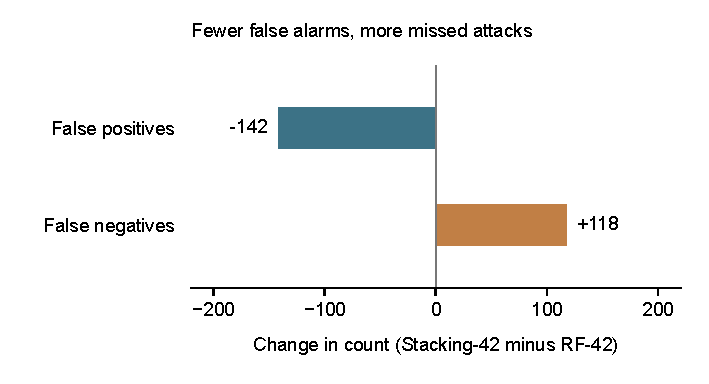
\includegraphics[width=0.82\textwidth]{../results/figures/p16_r05_error_tradeoff/error_tradeoff.pdf}
\caption{Chênh lệch số lượng lỗi Stacking-42 trừ RF-42 trên cùng official TEST: FP giảm 142 mẫu và FN tăng 118 mẫu. Số lượng quan sát trên benchmark cố định, không phải sai khác trung bình qua nhiều lần huấn luyện.}
\label{fig:delta-fp-fn}
\end{figure}

\section{Khoảng tin cậy và kiểm định cặp}
\label{sec:bat-dinh}

\begin{table}[htbp]
\centering
\small
\caption{Chênh lệch Stacking-42 trừ RF-42 và CI 95\% paired bootstrap đã lưu; 10\,000 lần lấy mẫu bootstrap từ các dòng benchmark. Đơn vị là độ chênh tuyệt đối trên thang 0--1.}
\label{tab:chenh-lech-ci}
\begin{tabular}{lrrr}
\hline
Chỉ số & $\Delta$ & CI dưới 95\% & CI trên 95\% \\
\hline
Macro-F1 & +0.000497 & -0.000312 & +0.001309 \\
MCC      & -0.000413 & -0.001938 & +0.001140 \\
FPR      & -0.003838 & -0.005243 & -0.002432 \\
FNR      & +0.002603 & +0.001853 & +0.003375 \\
\hline
\end{tabular}
\end{table}

Khoảng tin cậy của chênh lệch Macro-F1 và MCC chứa 0. Do đó, kết quả \emph{không cung cấp bằng chứng đủ mạnh cho ưu thế tổng thể} của Stacking-42 so với RF-42 trên hai thước đo này; điều này \emph{không} chứng minh hai mô hình tương đương thống kê. McNemar exact với hiệu chỉnh Holm trên \emph{đúng/sai tổng thể của các cặp dự đoán} cho $p_{\mathrm{Holm}}=0.468377$ trong cùng phép so sánh; McNemar không phải kiểm định trực tiếp chênh lệch Macro-F1.

CI của FPR nằm hoàn toàn phía âm và CI của FNR nằm hoàn toàn phía dương. Các khoảng tin cậy này phản ánh biến động do lấy mẫu lại \emph{các dòng benchmark đã lưu}, không phải độ ổn định qua các lần huấn luyện độc lập, session độc lập hay dữ liệu ngoài bộ UNSW-NB15. Hình forest plot và bảng số liệu nguồn được lưu trong \path{results/figures/p16_paired_effects_2026_10_16}.

\begin{figure}[htbp]
\centering
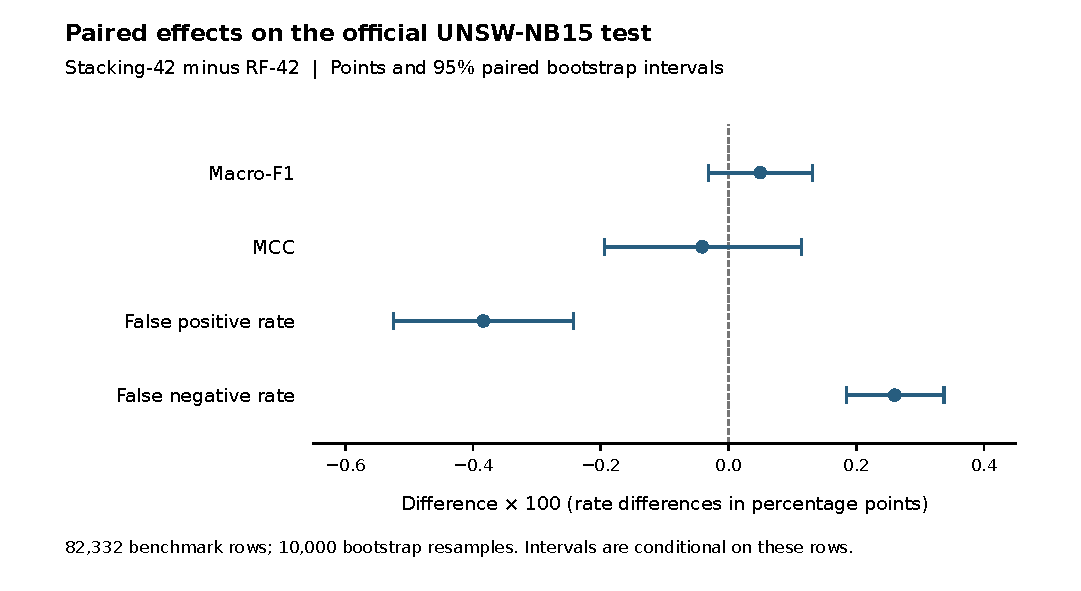
\includegraphics[width=0.95\textwidth]{../results/figures/p16_paired_effects_2026_10_16/paired_effects.pdf}
\caption{Bốn hiệu số Stacking-42 trừ RF-42 và CI 95\% paired bootstrap đã lưu. Giá trị trục ngang là hiệu số nhân 100 (không phải phần trăm thay đổi tương đối). CI của Macro-F1 và MCC chứa 0; FPR giảm, FNR tăng.}
\label{fig:paired-metrics}
\end{figure}

\section{Chi phí mô hình và số đặc trưng}
\label{sec:chi-phi}

\begin{table}[htbp]
\centering
\small
\caption{Chi phí được ghi nhận trong lần chạy lịch sử. Kích thước sử dụng đơn vị MiB (byte chia $1024^2$), không phải MB thập phân.}
\label{tab:chi-phi}
\begin{tabular}{lrrrr}
\hline
Pipeline & Số feature & Train (s) & Inference (ms/mẫu) & Size (MiB) \\
\hline
RF-42       & 42 & 371.244 & 0.008679 & 205.490 \\
Stacking-42 & 42 & 980.170 & 0.012445 & 206.216 \\
RF-17       & 17 & 57.255 & 0.003562 & 105.044 \\
\hline
\end{tabular}
\end{table}

Trong các số đo đã lưu, thời gian huấn luyện của RF-42 gấp khoảng 6,48 lần RF-17, và kích thước mô hình ước lượng của RF-17 thấp hơn khoảng 48,88\% so với RF-42. Các số liệu chỉ phản ánh \emph{chi phí quan sát của những cấu hình cụ thể trong lần chạy lịch sử}; chưa có phân bố thời gian qua nhiều lần huấn luyện và chưa có cơ sở dự báo thời gian trên thiết bị triển khai. Môi trường Python và thư viện tại thời điểm huấn luyện gốc chưa được xác định trực tiếp. Trường kích thước biểu diễn kết quả ước lượng serialize trong lần chạy, không chứng minh file mô hình cuối hiện tồn tại trên ổ đĩa.

\section{Phân tích lỗi theo họ tấn công}
\label{sec:attack-family-error}

\begin{table}[htbp]
\centering
\small
\caption{Số mẫu Attack thực bị dự đoán là Normal, phân nhóm theo \texttt{attack\_cat}; đây không phải đánh giá multiclass.}
\label{tab:attack-family}
\begin{tabular}{lrrrr}
\hline
Nhóm Attack & Số mẫu & FN RF-42 & FN Stack-42 & $\Delta$ FN \\
\hline
Fuzzers       & 6062  & 621 & 754 & +133 \\
Generic       & 18871 & 57  & 14  & -43 \\
Nhóm còn lại  & 20399 & 56  & 84  & +28 \\
\hline
Tổng Attack   & 45332 & 734 & 852 & +118 \\
\hline
\end{tabular}
\end{table}

Trên Fuzzers, Stacking-42 bỏ sót thêm 133 mẫu so với RF-42; trên Generic, Stacking-42 bỏ sót ít hơn 43 mẫu. Các đếm này mô tả tác động \emph{không đồng đều giữa các nhóm nhãn thật}, nhưng không chỉ ra cơ chế nhân quả của \texttt{sttl}, \texttt{proto} hay các feature khác. Những nhóm rất ít mẫu không cho phép khái quát chắc chắn về mọi tấn công ngoài benchmark. Tất cả phân tích lỗi được thực hiện hậu nghiệm trên prediction đã khóa, không được dùng để chỉnh ngưỡng dự đoán.

\section{Kiểm tra độ nhạy trên nhóm vector chưa trùng}
\label{sec:novel-vector}

\begin{table}[htbp]
\centering
\small
\caption{Macro-F1 trên official TEST và phần novel-vector của cùng official TEST. Novel-vector \emph{không} phải bộ dữ liệu kiểm thử độc lập.}
\label{tab:novel-vector}
\begin{tabular}{lrr}
\hline
Pipeline & Official TEST ($n=82332$) & Novel-vector ($n=73791$) \\
\hline
RF-42       & 0.863343 & 0.857473 \\
Stacking-42 & 0.863840 & 0.858125 \\
RF-17       & 0.860673 & 0.855723 \\
\hline
\end{tabular}
\end{table}

Cả ba pipeline có Macro-F1 thấp hơn trên nhóm novel-vector. Tập con này được xác định bằng cách loại những dòng TEST có vector 42 đặc trưng trùng với ít nhất một vector TRAIN; 8\,541 dòng TEST thuộc nhóm overlap theo cách định nghĩa này. Đây là một \emph{sensitivity analysis} trong cùng benchmark, không thay cho đánh giá external, temporal, day hoặc session split. Vì vậy, câu hỏi RQ4 về độ nhạy với \emph{split protocol} chưa được trả lời đầy đủ.

\section{Tổng hợp theo câu hỏi nghiên cứu và các giới hạn}
\label{sec:rq-limitations}

\textbf{RQ1 --- Hiệu quả ensemble:} chưa chứng minh cải thiện tổng thể hoặc ổn định qua nhiều lần huấn luyện của Stacking-42 so với RF-42. Kết quả cặp cho thấy dịch chuyển FP/FN rõ ràng trên holdout đã lưu.

\textbf{RQ2 --- Feature selection:} bảng so sánh RF-17 và RF-42 hỗ trợ mô tả đánh đổi hiệu năng--chi phí của \emph{cả pipeline}; không có đối chứng tách biệt tác động nhân quả của chỉ số feature vì cấu hình mô hình cũng khác nhau.

\textbf{RQ3 --- Complementarity:} các bảng OOF diversity và ensemble ở development hỗ trợ phân tích \emph{liên hệ mô tả} giữa sai số của base learners và kết quả kết hợp. Complementary errors không bảo đảm Stacking vượt mô hình đơn; các kết quả voting kém hơn vẫn phải được báo cáo.

\textbf{RQ4 --- Robustness:} novel-vector cho thấy một hướng kiểm tra độ nhạy nhưng không phải temporal/group/external validation. RQ4 mới được trả lời một phần.

\textbf{RQ5 phụ --- Class imbalance:} chưa có thí nghiệm controlled resampling so sánh matched, do đó không thể khẳng định SMOTE hay kỹ thuật sampling tương đương hiệu quả hoặc không hiệu quả trong nghiên cứu này.

\textbf{Giới hạn phương pháp:} (i) lựa chọn stable features trên toàn official TRAIN trước development CV có thể làm điểm CV lạc quan; (ii) lựa chọn/tuning meta-model chưa fully nested; (iii) có vector trùng giữa official TRAIN và TEST và các dòng network-flow không được chứng minh độc lập ở cấp session; (iv) paired bootstrap là trên dòng benchmark chứ không phải repeated-training stability; (v) môi trường training lịch sử chưa xác minh trực tiếp và chưa có final serialized model hợp lệ; (vi) không có kiểm tra external deployment/multiclass. Các giới hạn này không được xóa hoặc sửa kết quả official TEST sau khi đã quan sát.

\section{Kết luận chương}
Trong giới hạn official UNSW-NB15 holdout đã khóa, Stacking-42 làm giảm báo động giả nhưng đồng thời tăng số tấn công bị bỏ sót so với RF-42. Bằng chứng thống kê hiện có chưa xác nhận một cải thiện tổng thể về Macro-F1/MCC. RF-17 thể hiện khả năng giảm chi phí của một cấu hình pipeline khác với mức giảm nhỏ của Macro-F1. Giá trị khoa học hiện có nằm ở đối chiếu có truy vết, phân tích sai số, độ bất định và công bố giới hạn, thay vì tuyên bố một thuật toán ensemble mới hoặc khả năng triển khai ngoài benchmark đã được xác minh.

\section{Kết luận và định hướng phát triển}
\label{chap:ket-luan}

\subsection{Tổng kết kết quả}
Trên official UNSW-NB15 TEST gồm 82\,332 dòng, Stacking-42 đạt Macro-F1 khoảng 0.863840 so với 0.863343 của RF-42, trong khi MCC của Stacking-42 khoảng 0.750497, thấp hơn rất nhẹ so với 0.750910 của RF-42. Chênh lệch Macro-F1 Stacking-42 trừ RF-42 là khoảng $+0.000497$; khoảng tin cậy 95\% paired bootstrap đã lưu gồm 0. Những bằng chứng này \emph{không xác nhận ưu thế tổng thể} của Stacking-42 trên Macro-F1/MCC, và cũng không chứng minh hai mô hình tương đương về mặt thống kê.

Stacking-42 giảm 142 dự đoán báo động giả (FP) nhưng tăng 118 trường hợp bỏ sót tấn công (FN) so với RF-42. Phân tích hậu nghiệm cho thấy xu hướng lỗi khác nhau theo từng attack family: Stacking-42 có thêm 133 FN ở Fuzzers nhưng giảm 43 FN ở Generic. Những con số đó thuộc mô hình \emph{binary} và nhãn thật của các nhóm, không phải khả năng dự đoán multiclass hay bằng chứng về nguyên nhân từ các feature riêng lẻ.

RF-17 có Macro-F1 thấp hơn RF-42 một lượng nhỏ, đổi lại các số đo lịch sử cho thấy thời gian train ngắn hơn và ước lượng dung lượng mô hình giảm. Tuy nhiên, đây là so sánh \emph{pipeline-level} vì RF-17 không chỉ giảm đặc trưng mà còn thay đổi siêu tham số Random Forest. Không thể quy trực tiếp mọi thay đổi cho riêng Feature Selection.

\subsection{Đóng góp trong phạm vi đã chứng minh}
Đóng góp có thể bảo vệ ở thời điểm hiện tại là một chuỗi thực nghiệm trên benchmark có nguồn và cấu hình đóng băng, có kiểm toán dữ liệu, đối chiếu mô hình học máy đơn và ensemble, phân tích sai số bổ sung, khoảng tin cậy cho chênh lệch theo cặp, đánh đổi FP/FN và chi phí. Kết quả không thuận lợi của Voting và sự thiếu ưu thế rõ ràng của Stacking là thành phần của kết luận khoa học, không bị loại vì không hỗ trợ một giả thuyết chiến thắng.

Báo cáo cũng ghi nhận các giới hạn của phép đo: sai lệch tiềm tàng do Feature Selection trước development CV, meta tuning chưa fully nested, vector TRAIN/TEST bị trùng, benchmark flow có thể phụ thuộc lẫn nhau, thiếu temporal/external validation và thiếu bằng chứng ổn định qua các lần tái huấn luyện độc lập. Việc công khai những giới hạn này góp phần tránh suy diễn vượt mức về khả năng tổng quát hoặc tính mới của thuật toán.

\subsection{Công việc còn thiếu và hướng nghiên cứu}
Với RQ1, cần một nghiên cứu mới có nhiều lần huấn luyện độc lập, cùng tài nguyên và môi trường đã khóa để kiểm tra tính ổn định của hiệu số. Với RQ2, cần thí nghiệm matched và nested feature selection, giữ các tham số còn lại cố định để tách tác động của chính Feature Selection. Với RQ3, có thể kiểm tra giả thuyết về cơ chế bổ sung sai số bằng phân tích độc lập thay vì chỉ dùng profile hậu nghiệm. Với RQ4, cần nguồn có thông tin thời gian/session hoặc một external benchmark đáng tin cậy để đánh giá ngoài official split. Với RQ5, có thể thiết kế đối chứng resampling/class-weight bên trong training folds, nhưng không được dựa vào official TEST hiện tại để chọn phương án thắng.

Mã nguồn xử lý, huấn luyện và tổng hợp chỉ số tạo điều kiện kiểm tra quy trình thực nghiệm và tính nhất quán của các kết quả. Tuy nhiên, môi trường huấn luyện gốc chưa biết chắc, bản tái dựng full TRAIN chưa thực hiện và mô hình cuối dạng serialized chưa được xác minh. Do đó chưa thể công bố đã tái lập end-to-end hay có hệ thống phát hiện xâm nhập triển khai thực tế. Các mô hình được huấn luyện trên mẫu dữ liệu nhỏ để kiểm tra chương trình không đại diện cho mô hình cuối, vì vậy không thể dùng chúng để minh họa khả năng dự đoán tương ứng với bảng kết quả chính thức.

\subsection{Kết luận cuối}
Trong phạm vi benchmark và thí nghiệm đã khóa, kết quả chủ yếu nhấn mạnh nhu cầu so sánh Ensemble Learning một cách có kiểm soát, trình bày đầy đủ loại lỗi và độ bất định, thay vì chọn mô hình chỉ bởi một điểm Accuracy hoặc Macro-F1 nhỉnh hơn về mặt số học. Việc bổ sung Stacking đem lại một đánh đổi FP/FN cụ thể nhưng không xác lập ưu thế tổng thể trước RF-42. Các đóng góp có thể truy vết nằm ở cách đánh giá và diễn giải kết quả, không phải một cam kết superiority, novelty hoặc deployment chưa được kiểm chứng.


\clearpage
\bibliographystyle{plain}
\bibliography{references_verified,references_dataset_checked}
\end{document}
